\chapter{Theoretical Background}

\section{The Heat Equation}

The heat equation is a fundamental partial differential equation (PDE) that governs how temperature evolves in a given region over time. In its simplest form, we consider a one-dimensional case in which heat flows along a single spatial dimension:
\begin{align*}
  \frac{\partial u}{\partial t} & = \mu \frac{\partial^2 u}{\partial x^2} + f(u), \quad \left( x, t \right) \in \Omega \times \left(0, T\right) \tag{PDE} \\
                                &
  \begin{cases}
    u(x, 0) = u_0(x)  &                       \\
    u(0, t) = g(x, t) & x \in \partial \Omega \\
  \end{cases} \tag{BC}
\end{align*}\label{eq:heat_eq}

The equation describes how the temperature $u(x, t)$ at position $x$ and time $t$ evolves over time.

\paragraph{Diffusion and Reaction Terms}
The diffusion term $\mu \frac{\partial^2 u}{\partial x^2}$ describes how heat spreads through the material, while the reaction term $f(u)$ accounts for any heat sources or sinks in the system.

\paragraph{Initial and Boundary Conditions}
The initial temperature distribution $u_0(x)$ and boundary condition $g(x, t)$ specify the temperature at the start and where heat enters or leaves the system, respectively.

\paragraph{Parabolic PDE}
The heat equation is a \emph{parabolic} PDE describing how processes evolve over time. For numerical solutions, the spatial and temporal domains are discretized, and the solution is approximated at discrete points. Finite difference methods efficiently handle these discretizations, allowing accurate approximations of the evolving temperature.

\subsection{Discretization of the Heat Equation}
Discretizing the heat equation involves dividing the spatial domain $\Omega$ into $M$ equally spaced points and the temporal domain into $N$ steps. Each grid point is denoted by $(x_m, t_n)$, where $x_m = m h$ and $t_n = n k$.
The approximate temperature at each grid point is $U_m^n$, with $m = 0, \ldots, M$ and $n = 0, \ldots, N$.

\[
  U_m^n \approx u(x_m, t_n) \quad \text{for } (x_m, t_n) \in \mathbb{G}
\]


\begin{align*}
  \mathbb{G} & := \left\{ (x_m, t_n):\,
  \begin{cases}
    x_m = m h & h = \tfrac{L}{M},\; m = 0, \ldots, M \\
    t_n = n k & k = \tfrac{T}{N},\; n = 0, \ldots, N
  \end{cases}\right\}
\end{align*}\label{eq:grid_points}

Here, $L$ is the spatial domain length and $T$ the final time.
\begin{center}
  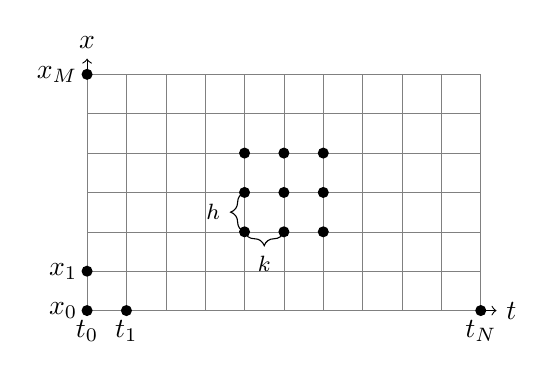
\begin{tikzpicture}

    % Axes
    \draw[->] (0,0) -- (5.2,0) node[right] {$t$};
    \draw[->] (0,0) -- (0,3.2) node[above] {$x$};

    % Grid points
    \draw[step=0.5cm,gray,very thin] (0,0) grid (5,3);

    \node[below] at (0,0) {$t_0$};
    \node[below] at (0.5,0) {$t_1$};
    \node[below] at (5,0) {$t_N$};
    \node[left] at (0,0) {$x_0$};
    \node[left] at (0,0.5) {$x_1$};
    \node[left] at (0,3) {$x_M$};

    % Add some key points with labels
    \foreach \x in {2,2.5,3} {
        \foreach \y in {1,1.5,2} {
            \fill (\x,\y) circle (2pt);
          }
      }

    % Add curly braces to show length k and h on axes
    \draw [decorate,decoration={brace,amplitude=5pt}]
    (2.5,1) -- (2,1) node [black,midway,yshift=-0.4cm] {\footnotesize $k$};
    \draw [decorate,decoration={brace,amplitude=5pt}]
    (2,1) -- (2,1.5) node [black,midway,xshift=-0.4cm] {\footnotesize $h$};

    % Add circles/points at nodes
    \fill (0,0) circle (2pt);
    \fill (0.5,0) circle (2pt);
    \fill (5,0) circle (2pt);
    \fill (0,0.5) circle (2pt);
    \fill (0,3) circle (2pt);

  \end{tikzpicture}
\end{center}

\begin{remark}{Constant Grid Spacing}{step_sizes}
  For simplicity, $h$ and $k$ are constant:
  \[
    x_{m+1} = x_m + h,\quad t_{n+1} = t_n + k.
  \]
\end{remark}


\section{Finite Difference Methods}

Finite difference methods approximate differential equations by replacing them with a system of algebraic equations on the chosen grid.
The heat equation is often solved with these methods for their simplicity and computational efficiency.

\subsection{Implicit Methods}
Time-dependent PDEs with diffusion terms often require implicit schemes to maintain stability, as explicit methods may become unstable for certain choices of $h$ and $k$.

\begin{lemma}{}{}
  % Lemma about why explicit methods can be unstable for diffusion-dominated problems.
\end{lemma}

\clearpage

\paragraph{Notation}
\begin{tabular}{ll}
  \textbf{Symbol}               & \textbf{Meaning}                       \\
  \hline                                                                 \\[-1em]
  \(u = u(x, t)\)               & Exact temperature distribution         \\
  \(u_m^n = u(x_m, t_n)\)       & Exact temperature at grid point        \\
  \(\mu\)                       & Diffusion coefficient                  \\
  \(f(u)\)                      & Reaction term                          \\
  \(u_0(x)\)                    & Initial temperature distribution       \\
  \(g(x, t)\)                   & Boundary condition                     \\
  \(\Omega\)                    & Spatial domain                         \\
  \(\partial \Omega\)           & Boundary of spatial domain             \\
  \hline                                                                 \\[-1em]
  \(U_m^n \approx u(x_m, t_n)\) & Numerical approximation of temperature \\
  \(x_m = m h\)                 & Spatial grid points                    \\
  \(t_n = n k\)                 & Temporal grid points                   \\
  \(h = L/M\)                   & Spatial step size                      \\
  \(k =T/N\)                    & Temporal step size                     \\
  \(L\)                         & Spatial domain length                  \\
  \(T\)                         & Final time                             \\
  \(M\)                         & Number of spatial grid points          \\
  \(N\)                         & Number of temporal grid points         \\
  \(\mathbb{G}\)                & Set of all grid points                 \\
  \hline
\end{tabular}
